\documentclass[10pt]{article}
\usepackage[T1]{fontenc}
\usepackage[utf8]{inputenc}
\usepackage{lmodern}
\usepackage[a4paper,margin=24mm]{geometry}
\usepackage{amsmath,amssymb,booktabs,graphicx,array}
\usepackage{xcolor}
\definecolor{flm}{HTML}{A74C20}
\usepackage[colorlinks=true,linkcolor=flm,citecolor=flm,urlcolor=flm]{hyperref}
\usepackage{microtype}
\setlength{\parskip}{5pt}
\setlength{\parindent}{0pt}
\setlength{\emergencystretch}{2em}
\renewcommand{\arraystretch}{1.15}
\graphicspath{{figures/}}
\newcommand{\code}[1]{\texttt{\detokenize{#1}}}

\newcommand{\WiringRows}{%
BPTT & 100.00 & 66.67 & 63.02 & 76.04 \\
Fixed core & 86.46 & 55.73 & 63.15 & 44.53 \\
Eligibility & 83.33 & 50.00 & 53.52 & 57.03 \\
No trace history & 50.00 & 66.93 & 57.68 & 55.34 \\
Reward + eligibility & 50.00 & 50.00 & 66.67 & 50.00 \\
}
\newcommand{\CueMeasured}{100.00}
\newcommand{\CueNull}{66.67}
\newcommand{\ContextMeasured}{63.02}
\newcommand{\ContextNull}{76.04}
\newcommand{\GradientRows}{%
0 & 0.452 & 0.428 & 0.893 & 0.759 \\
300 & 0.361 & 0.320 & 0.486 & 0.363 \\
600 & 0.332 & 0.196 & 0.585 & 0.422 \\
900 & 0.402 & 0.127 & 0.564 & 0.426 \\
}

\hypersetup{pdftitle={FLM: Wiring Controls, Context and Local Credit},pdfauthor={Kuber Mehta},pdflang={en}}
\title{\textbf{FLM: Wiring Controls, Context and Local Credit}\\[6pt]\large A sixty-run diagnostic study with mixed topology effects}
\author{Kuber Mehta\\\href{https://flm.kuber.studio}{flm.kuber.studio}}
\date{12 September 2026 --- status-updated working note}
\begin{document}
\maketitle
\begin{abstract}
Does measured wiring help the computation performed by an artificial fly-wired
network? We compare five learning rules on measured and constrained-randomized
graphs in two delayed-choice tasks. Sixty fixed-budget runs share initial
parameters and sensory streams within each task and each of three seed pairs. At the final
48-frame cue probe, full backpropagation through time (BPTT) averages
\CueMeasured\% with measured wiring and \CueNull\% with randomized wiring.
For the harder delayed-context task at delay eight, the ordering reverses:
\ContextMeasured\% versus \ContextNull\%. Gradient probes quantify departures
of local eligibility estimates from exact temporal credit. These mixed results
establish no general anatomical or local-learning advantage. This is a small
artificial-task study. The separate, now-completed WikiText topology report
finds no measured-wiring advantage for its selected language subset;
a distinct 128-fit selection follow-up has no held-out result yet.
\end{abstract}

\section{The comparison that is needed}
FLM uses measured neural edges as a fixed prior for a trainable recurrent rate
network. Successful task learning alone does not show that measured wiring is
useful: the same machinery may work as well on an appropriate random graph.
Connectome-constrained visual-system evidence concerns different predictions
\cite{lappalainen}. A recent flyvis preprint illustrates how initialization and
null-model choices can weaken an apparent topology effect \cite{dhiman2026}.
Neither source establishes an FLM language advantage.

\begin{figure}[h]\centering
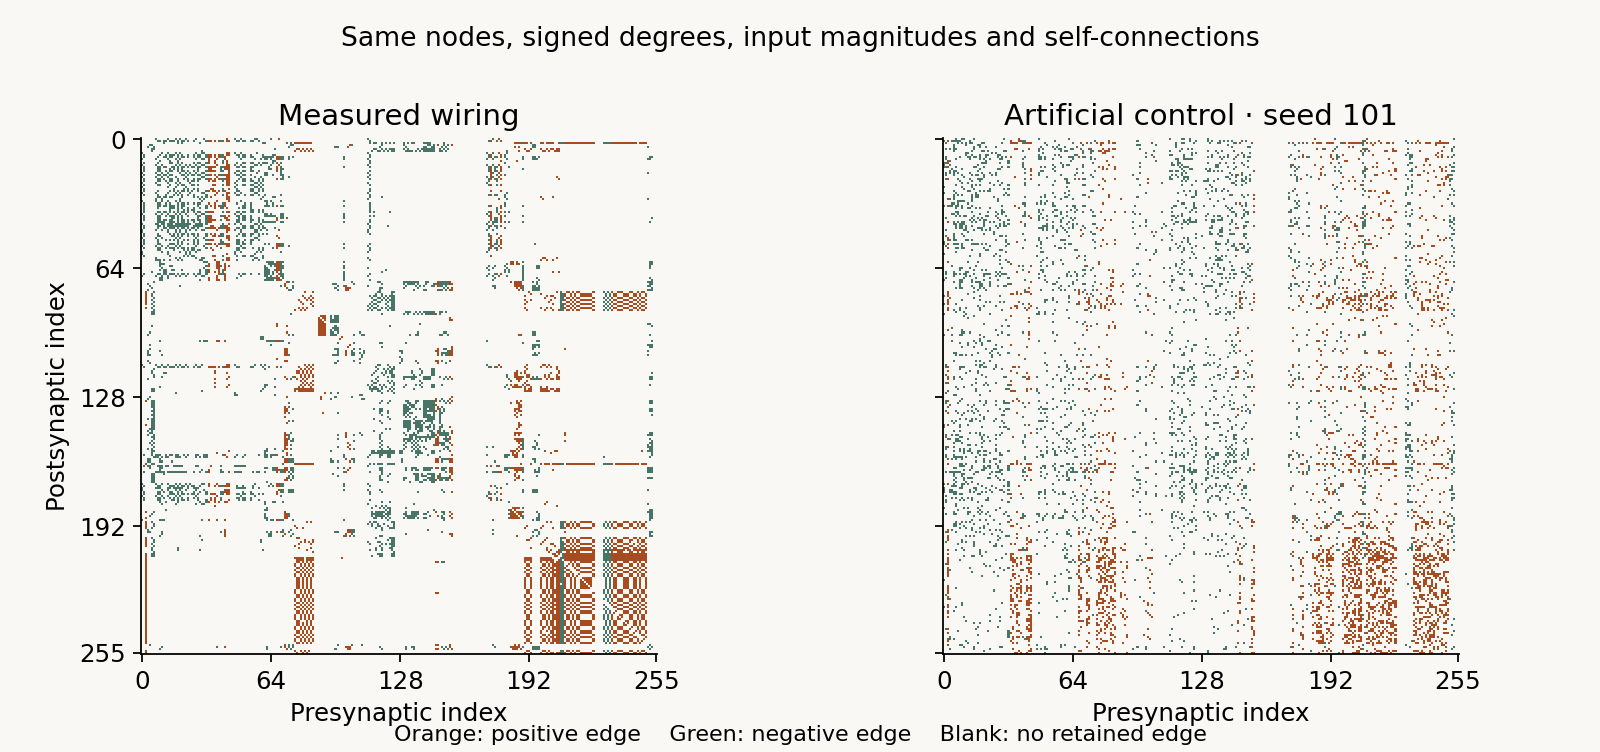
\includegraphics[width=.93\textwidth]{wiring-matrix.png}
\caption{Measured 256-neuron subset and one artificial control, in the same node
order. Rows are postsynaptic and columns presynaptic. The control preserves
degrees, input signs and magnitudes, and original self edges. New edges are
artificial; their transferred contact values are not measured new synapses.}
\end{figure}

\newpage
\section{Matched graph and learning machinery}
The measured graph retains 256 central intrinsic MaleCNS neuron identities,
6,678 directed edges and 32 output pools \cite{malecns}. It is a different subset
from FLM's 1,024-neuron language core. The four sensory inputs and two-action
readout are engineered, not biological sensory or descending pathways. All
models allocate 8,729 parameters.

Each null begins from the measured graph. A double-edge swap
$(i,j),(k,l)\mapsto(i,l),(k,j)$ exchanges presynaptic endpoints only when sources
$j,l$ have the same assumed neurotransmitter sign. Reject duplicates, new self
edges and unchanged proposals. Preserve every original self edge at its weight;
keep all other array slots except the source index unchanged. Each chain accepts
ten swaps per edge. This extends a degree-preserving null construction
\cite{maslov2002} with explicit sign and self-edge constraints.

Thus every neuron's directed in/out degree, target-wise signed incoming
weight/contact multiset, node order, coordinates and pool membership match.
Outgoing weighted strength, distance, reciprocity and higher motifs need not
match. The three nulls retain approximately 23\% of original edges. Reciprocal
off-diagonal edges fall from 67.96\% to 14.74--15.31\%. Finite chains do not
establish uniform sampling or adequate mixing over all allowed graphs.

The normalized rate recurrence is
\begin{align}
W_{ij}&=\frac{b_{ij}\exp(\theta_{ij})}{\sum_k|b_{ik}\exp(\theta_{ik})|},\quad
z_t=\tanh(Ax_t+b+gWh_{t-1}),\\
h_t&=(1-\alpha)\odot h_{t-1}+\alpha\odot z_t,\qquad
s_t=(1-\beta)\odot s_{t-1}+\beta\odot h_t.
\end{align}
Signs of $b$ are fixed; edge logits are bounded to $[-3,3]$. Sigmoids bound
$\alpha\in(.05,.95)$, $\beta\in(.002,.100)$ and $g\in(.05,3)$. Pooled fast and
slow states pass through LayerNorm and a binary readout.

Five rules use SGD at .03, batch eight, clipping at one, and no momentum or
weight decay: full BPTT; fixed-core readout learning (258 effective trainable
parameters); supervised forward eligibility; the same approximation with trace
history cleared each frame; and reward-modulated eligibility. The forward rules
retain direct temporal derivatives but omit indirect temporal routes through
other neurons. Instantaneous readout derivatives supply the learning signal.
The normalized-edge direct derivative includes
$\partial (Wh)_i/\partial\theta_{ij}=W_{ij}h_j-|W_{ij}|(Wh)_i$.
Eligibility is motivated by prior work \cite{bellec}, not a new property unique
to fly wiring. This rate-network approximation is not a spiking e-prop reproduction.

\section{Tasks, phases and experimental units}
The cue task has two cue frames, a sampled delay $D\in\{4,\ldots,12\}$ and one
query frame. The context task adds two later context frames and another delay:
$T=2D+5$. The answer is cue XOR context. Gaussian distractor input (SD .2)
occupies another channel throughout. Batches balance the binary cues or all four
cue/context combinations. States reset each episode; weights persist.

All runs train the original rule for updates 1--300, its inverse for 301--600,
then the original for 601--900: 7,200 episodes. No phase flag is supplied.
Model seeds 17/29/41 are paired with null seeds 101/103/107. The design is
two tasks $\times$ two topologies $\times$ five rules $\times$ three seed pairs.
Graph and initialization variation are \emph{not} independently crossed here.
The 15 measured-cue conditions reproduce the earlier trained tensors and
sample-stream hashes exactly; they are bridges, not extra replications.

\newpage
\section{Results: topology effects change with the task}
Fixed panels contain 256 balanced episodes at delays 4, 8, 12, 24 and 48, measured
initially and every 100 updates. They are reused diagnostics, not untouched test
data or checkpoint-selection criteria. Every run finishes at 900; no favorable
seed or checkpoint is selected. Equal episodes across tasks do not mean equal
numbers of sensory frames or equal computation.

\begin{table}[h]\centering\small
\caption{Final accuracy (\%), three-seed means. These two declared panels show
a change in ordering; all 3,000 seed-level observations remain available.}
\begin{tabular}{lrrrr}\toprule
& \multicolumn{2}{c}{Cue, delay 48} & \multicolumn{2}{c}{Context, delay 8}\\
Learning rule & Measured & Rewired & Measured & Rewired\\\midrule
\WiringRows
\bottomrule\end{tabular}
\end{table}

\begin{figure}[h]\centering
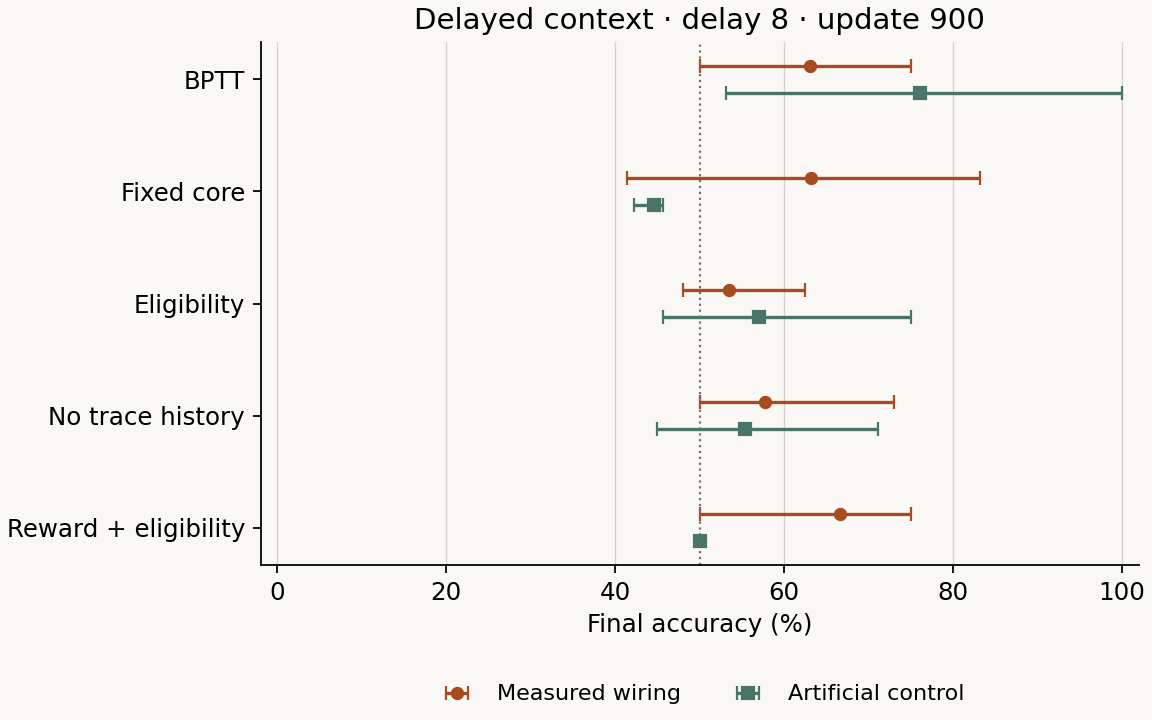
\includegraphics[width=.87\textwidth]{wiring-context-delay8.png}
\caption{Final context accuracy at delay eight. Markers are means; bars span
the observed three-seed range, not a confidence interval. Chance is 50\%.
Wide ranges preclude a robust ordering based on the mean alone.}
\end{figure}

The cue task gives measured wiring an advantage for some long-delay conditions,
including BPTT, fixed-core and supervised eligibility. That observation does
not generalize to the context task. BPTT's measured-minus-null contrast at
delay eight averages $-13.02$ percentage points, with paired seed differences
from $-50.00$ to $+10.94$. The measured fixed-core mean instead exceeds its null
mean by 18.62 points in that panel, again with a seed-dependent sign.

Supervised eligibility does not consistently outperform its no-history or
fixed-core alternatives. Most final context conditions approach chance at
delay 48; measured fixed-core accuracy averages 57.55\%. Reward eligibility's
binary correctness feedback also reveals the alternative action's correctness,
so this assay does not establish learning from strictly less target information.
The complete delays, phases, probabilities and per-seed losses are published.

\newpage
\section{How far is local credit from the exact gradient?}
At updates 0, 300, 600 and 900, fixed eight-episode delay-eight probes compare
the exact supervised core gradient $g$ with an approximate gradient $\hat g$.
Copied float64 models ensure that diagnostics never update trained weights or
RNG state. The archive reports cosine $g^\top\hat g/(\|g\|\|\hat g\|)$, relative
L2 error, norms and sign agreement for all six core parameter groups and their
concatenation. Undefined ratios remain explicit.

\begin{figure}[h]\centering
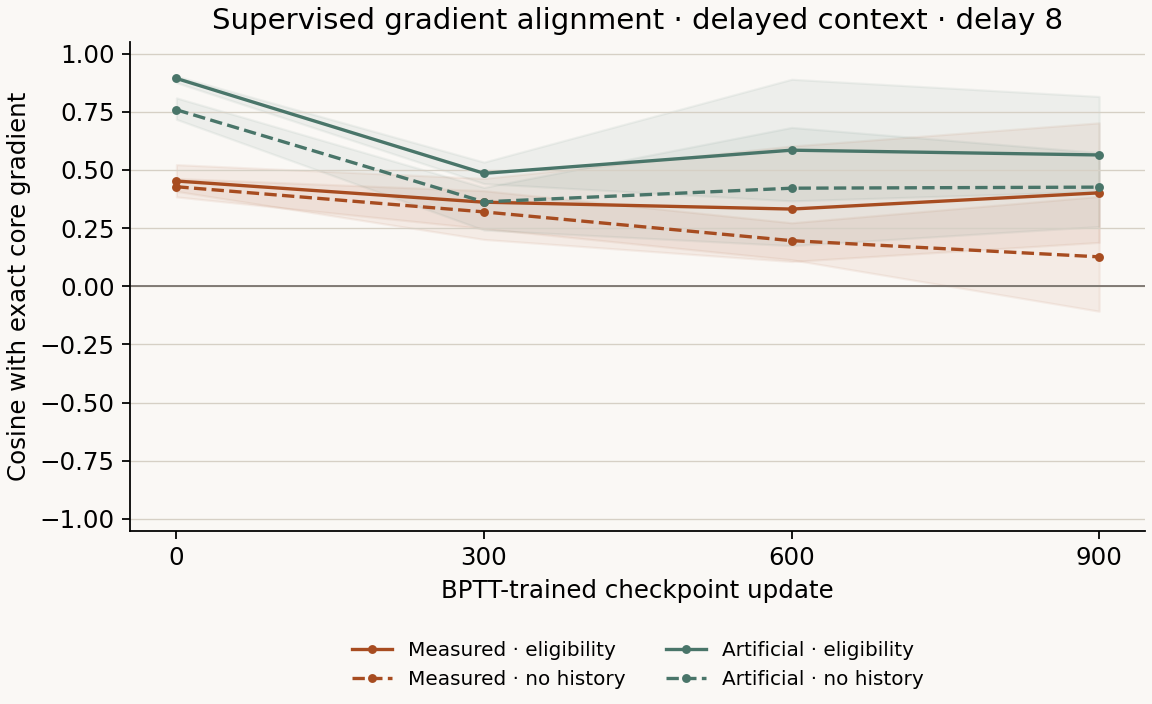
\includegraphics[width=.87\textwidth]{wiring-gradient-alignment.png}
\caption{Context task, BPTT-trained checkpoints. Exact-versus-approximate core
gradient cosine; lines are seed means and shading their range. This is a
supervised derivative diagnostic, including when separately inspecting
reward-trained networks. It is not a reward-gradient verification.}
\end{figure}

Local credit is not exact BPTT and its alignment depends on graph and training
state. Better cosine is not sufficient to predict better learning: magnitude,
optimization trajectories and the task also matter. Reward-driven models are
evaluated with the same supervised probe for comparability, not by equating
cross-entropy with their training objective.

\section{Limits, language follow-up and reproducibility}
There is no general anatomical advantage established by these diagnostics.
Only one small subset, three paired seeds, two artificial tasks and one fixed
learning budget were tested. Random controls retain substantial anatomical
information. Repeated probes are not independent samples, and seed ranges are
not uncertainty intervals for populations of graphs or tasks. The body replay
study is separate; these results imply neither animal learning nor learned gait.

The language follow-up uses three 1,024-neuron null graphs \emph{crossed} with
training seeds 42/43, plus two measured-graph models retrained without slow
state, under the original WikiText budget. All eight new runs and ten checkpoint selections completed before
new-control test scoring. The completed report finds no measured-wiring
advantage in that subset and setup; retaining slow state helps against
retrained no-slow controls. These results are reported separately in the
main FLM paper. The active 128-fit selection study is a distinct follow-up,
with validation and held-out results pending. The original main-language test scores were already
inspected, so the extension is exploratory.

The repository describes graph, reference-run and environment prerequisites.
Reproduce training and then verify the records with:
\begin{quote}\code{python -m flm.wiring_study}\\
\code{python -m flm.wiring_report}\end{quote}
The website provides the declared protocol, graph identities, every retained
prediction, CSVs and a 71-entry archive. Tables here are generated from the
verified complete records.

\begingroup\footnotesize
\bibliographystyle{unsrt}\bibliography{references}
\endgroup
\end{document}
